\documentclass[11pt, a4paper]{article}

% --- Ρυθμίσεις για XeLaTeX & Ελληνικά ---
\usepackage{fontspec}
\setmainfont{CMU Serif} 
\usepackage[english, main=greek]{babel}

% --- ΠΑΚΕΤΑ ΓΙΑ ΤΟ "THEME" ---
\usepackage[table, xcdraw]{xcolor} 
\usepackage{geometry}
\geometry{top=3cm, bottom=3cm, left=2.5cm, right=2.5cm}
\usepackage{graphicx}
\usepackage{enumitem}
\usepackage{tabularx}
\usepackage{svg}
\usepackage{float} 
\usepackage{tcolorbox} % [ΠΡΟΣΘΗΚΗ] Για τα όμορφα κουτιά πληροφοριών

% --- ΟΡΙΣΜΟΣ ΧΡΩΜΑΤΟΣ ΘΕΜΑΤΟΣ (Deep Blue) ---
\definecolor{PrimaryColor}{RGB}{0, 82, 155} 
\definecolor{SecondaryColor}{RGB}{100, 100, 100}
\definecolor{LightBlue}{RGB}{235, 245, 255} % Για το background του Info Box

% --- STYLING: Links & Bullets ---
\usepackage{hyperref}
\hypersetup{
    colorlinks=true,
    linkcolor=PrimaryColor, 
    urlcolor=PrimaryColor,
    citecolor=PrimaryColor
}

% [ΠΡΟΣΘΗΚΗ] Χρωματιστά bullets και αριθμοί στις λίστες
\newcommand{\cbullet}{\textcolor{PrimaryColor}{\textbullet}}
\setlist[itemize]{label=\cbullet}
\setlist[enumerate]{label=\textbf{\textcolor{PrimaryColor}{\arabic*.}}}

% --- STYLING: Section Titles ---
\usepackage{titlesec}
\titleformat{\section}{\Large\bfseries\color{PrimaryColor}}{\thesection}{1em}{}[\color{PrimaryColor}\titlerule]
\titleformat{\subsection}{\large\bfseries\color{PrimaryColor}}{\thesubsection}{1em}{}

% --- STYLING: Headers & Footers ---
\usepackage{fancyhdr}
\pagestyle{fancy}
\fancyhf{} 
\lhead{\textcolor{SecondaryColor}{\small Map-Reduce on Kubernetes}} 
\rhead{\textcolor{SecondaryColor}{\small Design Document}} 
\cfoot{\textcolor{SecondaryColor}{\thepage}} 
\renewcommand{\headrulewidth}{0.4pt}
\renewcommand{\headrule}{\hbox to\headwidth{\color{PrimaryColor}\leaders\hrule height \headrulewidth\hfill}} 

% --- Αποτροπή "σπασίματος" παραγράφων ---
\widowpenalty=10000
\clubpenalty=10000
\displaywidowpenalty=10000

\begin{document}
\sloppy 

% ==========================================
% CUSTOM ΕΞΩΦΥΛΛΟ (Title Page)
% ==========================================
\begin{titlepage}
    \centering
    \vspace*{3cm}
    
    {\Huge \textbf{\color{PrimaryColor} Design Document}}\\[1cm]
    {\LARGE Implementation of Map-Reduce on Kubernetes}\\[2.5cm]
    
    {\Large \textbf{INF-419 Principles of Distributed Systems}}\\[0.5cm]
    {\large Καθηγητής: Βασίλης Σαμολαδάς}\\[2.5cm]
    
    \vfill
    
    \begin{flushleft}
        {\large \textbf{\color{PrimaryColor} Ομάδα Ανάπτυξης:}}\\
        \vspace{0.3cm}
        \large Κρητικάκης Μάριος (2020030213) \\
    \end{flushleft}
    
    \vspace{2cm}
    {\large \textbf{22 Μαρτίου 2026}}
\end{titlepage}
% ==========================================

\newpage
\thispagestyle{empty} 
% --- ΟΜΟΡΦΟΤΕΡΑ ΠΕΡΙΕΧΟΜΕΝΑ ---
{
  % 1. Κάνουμε τα links μαύρα μόνο για αυτή την ενότητα
  \hypersetup{linkcolor=black} 
  
  % 2. Δίνουμε λίγο κάθετο "αέρα" ανάμεσα στα sections για να μη φαίνονται στριμωγμένα
  \setlength{\baselineskip}{1.5em} 
  
  \tableofcontents
}
% ------------------------------

\newpage
\setcounter{page}{1}

\section{Επιλογή Εργαλείων (Programming Tools)}
Η αρχιτεκτονική του συστήματος απαιτεί τεχνολογίες που προσφέρουν υψηλή διαθεσιμότητα, οριζόντια κλιμάκωση και ανθεκτικότητα. Η επιλογή της τεχνολογικής στοίβας (tech stack) έγινε με βάση τα παρακάτω αυστηρά κριτήρια:

\begin{itemize}
    \item \textbf{Οικοσύστημα Python:} Η επιλογή της Python ξεπερνά την απλή ταχύτητα ανάπτυξης. Η γλώσσα επιλέχθηκε στρατηγικά λόγω της εγγενούς υποστήριξης για data serialization (\texttt{JSON}, \texttt{Pickle}), της ευκολίας δυναμικής φόρτωσης κώδικα (απαραίτητο για να τρέχουν οι Workers τον κώδικα που ανεβάζει ο χρήστης) και της ύπαρξης στιβαρών βιβλιοθηκών όπως η \texttt{boto3} για επικοινωνία με S3 APIs. Για τα RESTful endpoints, εργαλεία όπως το FastAPI/Flask προσφέρουν ασύγχρονη διαχείριση I/O, ιδανική για microservices.

    \item \textbf{Identity \& Access Management - Keycloak:} Αντί για την υλοποίηση ενός απλού custom JWT generator, επιλέχθηκε το Keycloak. Πρόκειται για μια production-grade λύση που προσφέρει εγγενώς OAuth2.0/OpenID Connect. Η επιλογή αυτή εξασφαλίζει ισχυρό Role-Based Access Control (RBAC), διαχωρίζοντας απόλυτα τα δικαιώματα του Administrator από τους απλούς χρήστες, χωρίς να επιβαρύνεται ο κώδικας των microservices με την πολυπλοκότητα της κρυπτογραφίας των tokens.

    \item \textbf{Distributed Data Service (DDS) - PostgreSQL:} Το State του συστήματος (ποιο job τρέχει, ποια tasks απέτυχαν) είναι το πιο κρίσιμο σημείο αποτυχίας (Single Point of Failure). Επιλέξαμε PostgreSQL έναντι μιας NoSQL λύσης, καθώς απαιτούμε αυστηρή συνέπεια δεδομένων (Strict Consistency).
\end{itemize}

\begin{tcolorbox}[colback=LightBlue, colframe=PrimaryColor, title=\textbf{Σχεδιαστική Απόφαση: ACID Transactions vs Eventual Consistency}, arc=4mm]
Κατά τη φάση του Synchronization (όταν ο Manager ελέγχει αν όλα τα Map tasks έχουν ολοκληρωθεί για να ξεκινήσει το Reduce), η παραμικρή ασυνέπεια στα δεδομένα (Eventual Consistency μιας NoSQL) θα μπορούσε να οδηγήσει σε πρόωρη έναρξη των Reducers. Οι ACID ιδιότητες της PostgreSQL εγγυώνται ότι ο Manager βλέπει πάντα το πραγματικό, συγχρονισμένο State του cluster.
\end{tcolorbox}

\begin{itemize}
    \item \textbf{Shared File System - MinIO:} Το MinIO παρέχει συμβατότητα με το Amazon S3 API. Αντί να χρησιμοποιήσουμε ένα παραδοσιακό κοινόχρηστο σύστημα αρχείων (όπως NFS), στραφήκαμε στο Object Storage. Η αρχιτεκτονική του Map-Reduce βασίζεται σε εγγραφές χωρίς μεταβολές (append-only/immutable data). Το Object Storage υπερτερεί σε τέτοια workloads προσφέροντας τεράστιο throughput κατά το κατανεμημένο διάβασμα (Map phase) και γράψιμο (Reduce phase).
\end{itemize}

\begin{tcolorbox}[colback=LightBlue, colframe=PrimaryColor, title=\textbf{Σχεδιαστική Απόφαση: Αποφυγή POSIX Locks}, arc=4mm]
Η χρήση ενός Object Store όπως το MinIO εξαλείφει το overhead των POSIX file locks που θα αντιμετωπίζαμε με ένα παραδοσιακό NFS, επιτρέποντας σε χιλιάδες Workers να γράφουν τα ενδιάμεσα (intermediate) αρχεία τους ταυτόχρονα, χωρίς κανένα file-system level contention.
\end{tcolorbox}

\begin{itemize}
    \item \textbf{Ενορχήστρωση - Kubernetes (Minikube):} Το Kubernetes δεν είναι απλά ο host των containers, αλλά ενεργό μέρος της λογικής του συστήματος. Χρησιμοποιώντας τα \texttt{batch/v1 Jobs} του Kubernetes για τους Workers, εκμεταλλευόμαστε τους εγγενείς μηχανισμούς fault tolerance. Εάν ένα Worker pod τερματιστεί λόγω έλλειψης μνήμης (OOM) ή hardware failure, ο Kube-Controller Manager αναλαμβάνει αυτόματα την επανεκκίνησή του (βάσει του \texttt{backoffLimit}), αφαιρώντας αυτό το βάρος από την υλοποίηση του δικού μας Manager Service.
\end{itemize}

\section{Αρχιτεκτονική Microservices \& API}
Το σύστημα υλοποιεί την αρχιτεκτονική 3 επιπέδων και αποτελείται από τις εξής υπηρεσίες (microservices):
\begin{itemize}
    \item \textbf{UI Service:} Stateless υπηρεσία (Deployment) που παρέχει το API για τα CLI commands (jobs, admin).
    \item \textbf{Auth Service:} Διαχειρίζεται την ταυτοποίηση των χρηστών. Κάθε αίτημα στο UI Service συνοδεύεται από το token που εκδίδει αυτή η υπηρεσία.
    \item \textbf{Manager Service:} Η κεντρική υπηρεσία (StatefulSet) που συντονίζει την εκτέλεση των jobs, διαβάζει τα δεδομένα από το DDS και δημιουργεί τους Workers.
    \item \textbf{Workers:} Τα nodes (Kubernetes Jobs) που εκτελούν τους Mappers και Reducers.
\end{itemize}

\subsection{Προδιαγραφές Διεπαφών (API Specifications)}
Η επικοινωνία μεταξύ των microservices γίνεται μέσω RESTful APIs, με τα δεδομένα να ανταλλάσσονται σε μορφή JSON.
\begin{description}
    \item[UI Service API (Public):] \hfill
    \begin{itemize}
        \item \texttt{POST /api/v1/jobs}: Υποβολή νέου Map-Reduce job. Δέχεται το path των δεδομένων και τον κώδικα. Επιστρέφει \texttt{job\_id}.
        \item \texttt{GET /api/v1/jobs/\{id\}}: Επιστρέφει την κατάσταση ενός job.
        \item \texttt{POST /api/v1/admin/users}: Δημιουργία νέου χρήστη (απαιτεί Admin role).
    \end{itemize} 

    \item[Auth Service API (Public/Internal):] \hfill
    \begin{itemize}
        \item \texttt{POST /auth/login}: Δέχεται credentials και επιστρέφει ένα JWT (JSON Web Token) για το Single Sign-On.
        \item \texttt{POST /auth/validate}: Εσωτερικό endpoint που καλεί το UI service για να επιβεβαιώσει την εγκυρότητα του token.
    \end{itemize} 
    
    \item[Manager Service API (Internal):] \hfill
    \begin{itemize}
        \item \texttt{POST /internal/jobs}: Το UI service προωθεί εδώ τα επικυρωμένα jobs για να μπουν στην ουρά αναμονής.
        \item \texttt{PUT /internal/tasks/\{task\_id\}/status}: Οι Workers καλούν αυτό το endpoint για να αναφέρουν την πρόοδό τους και να καταγραφεί στο DDS.
    \end{itemize}
\end{description}

\section{Κύρια Use Cases}

\subsection{Υποβολή Job (Submit Job)}
Ο χρήστης κάνει αυθεντικοποίηση (login) και λαμβάνει ένα token. Στη συνέχεια, μέσω του CLI, στέλνει τα αρχεία κώδικα (mapper/reducer) και τα δεδομένα. Το UI service προωθεί την εντολή στον Manager, ο οποίος αποθηκεύει το νέο Job στο DDS με κατάσταση \texttt{PENDING}.

\begin{figure}[H] 
    \centering
    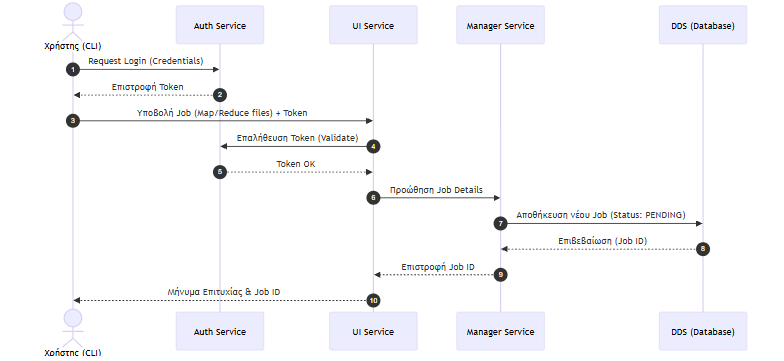
\includegraphics[width=0.9\textwidth]{diagrams/SubmitJob.png}
    \caption{Διάγραμμα Αλληλουχίας για την Υποβολή Job}\label{fig:submit_job}
\end{figure}

\subsection{Εκτέλεση Υπολογισμού (Run Compute Job)}
Ο Manager Service ανιχνεύει τα \texttt{PENDING} jobs. Για κάθε job, κάνει spawn τα αντίστοιχα Kubernetes Jobs (Workers). Οι Workers κατεβάζουν τα δεδομένα από το MinIO, εκτελούν τη συνάρτηση (Map ή Reduce), γράφουν τα αποτελέσματα πίσω στο MinIO και ενημερώνουν τον Manager για την ολοκλήρωση.

\begin{figure}[H] 
    \centering
    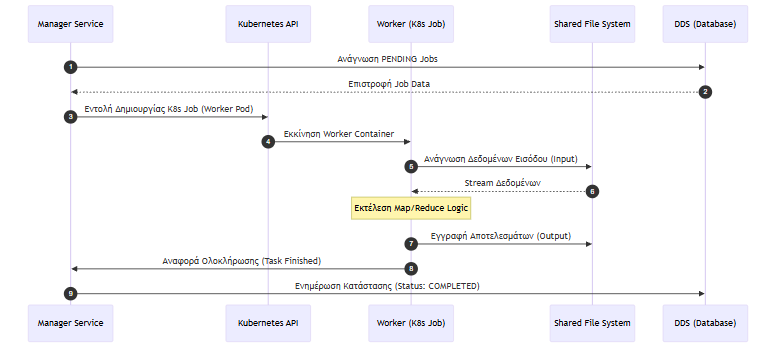
\includegraphics[width=0.9\textwidth]{diagrams/ExecuteJob.png}
    \caption{Διάγραμμα Αλληλουχίας για την Εκτέλεση του Job}\label{fig:execute_job}
\end{figure}

\newpage % [ΑΛΛΑΓΗ] Καθαρή αλλαγή σελίδας εδώ

\section{Οργάνωση Αποθηκευτικού Χώρου (Storage Namespaces)}
Για την αποφυγή συγκρούσεων (collisions) κατά την ταυτόχρονη εκτέλεση πολλαπλών Map-Reduce jobs, ορίστηκε μια αυστηρή ιεραρχία ονοματοδοσίας (namespace hierarchy) στο MinIO. Κάθε job διαθέτει το δικό του απομονωμένο περιβάλλον αποθήκευσης:

\begin{itemize}
    \item \texttt{s3://mapreduce-data/\{user\_id\}/\{job\_id\}/input/}: Φάκελος όπου ο χρήστης ανεβάζει το αρχικό αρχείο δεδομένων.
    \item \texttt{s3://mapreduce-data/\{user\_id\}/\{job\_id\}/code/}: Αποθήκευση των αρχείων \texttt{mapper.py} και \texttt{reducer.py}.
    \item \texttt{s3://mapreduce-data/\{user\_id\}/\{job\_id\}/intermediate/}: Προσωρινός φάκελος όπου οι Map Workers αποθηκεύουν τα ενδιάμεσα key-value pairs.
    \item \texttt{s3://mapreduce-data/\{user\_id\}/\{job\_id\}/output/}: Εδώ οι Reduce Workers γράφουν τα τελικά αποτελέσματα.
\end{itemize}

% [ΠΡΟΣΘΗΚΗ] Επαγγελματικό Info Box
\begin{tcolorbox}[colback=LightBlue, colframe=PrimaryColor, title=\textbf{Σχεδιαστική Απόφαση: Απομόνωση Δεδομένων}, arc=4mm]
Η χρήση μοναδικών S3 paths ανά \texttt{job\_id} διασφαλίζει ότι το σύστημα είναι οριζόντια κλιμακώσιμο (horizontally scalable) χωρίς τον κίνδυνο race conditions κατά την εγγραφή των ενδιάμεσων αρχείων από τους πολλαπλούς Workers.
\end{tcolorbox}

\section{Μηχανισμός Shuffling \& Ροή Δεδομένων}
Η διαδικασία επεξεργασίας ενός job χωρίζεται σε τρεις διακριτές φάσεις τις οποίες ενορχηστρώνει ο Manager Service:

\begin{enumerate}
    \item \textbf{Map Phase:} Ο Manager χωρίζει το input αρχείο σε $M$ λογικά partitions και δημιουργεί $M$ αντίστοιχα Worker Pods. Κάθε Mapper παράγει ενδιάμεσα \texttt{(key, value)} pairs, τα οποία κατακερματίζονται (μέσω $hash(key) \pmod R$) σε $R$ περιοχές.
    
    \item \textbf{Synchronization (Barrier):} Ο Manager Service παρακολουθεί τη βάση δεδομένων (DDS). Μόνο όταν \textbf{όλα} τα Map tasks περάσουν σε κατάσταση \texttt{COMPLETED}, το σύστημα προχωράει στην επόμενη φάση.
    
    \item \textbf{Reduce Phase:} Ο Manager δημιουργεί $R$ νέα Worker Pods (Reducers). Ο Reducer με id $r$ αναζητά στο MinIO όλα τα αρχεία της μορφής \texttt{intermediate/*\_part\_\{r\}.json} (η κατανεμημένη φάση του Shuffle). Κατόπιν, εκτελεί τον κώδικα και γράφει το τελικό αποτέλεσμα.
\end{enumerate}

\newpage % [ΑΛΛΑΓΗ] Καθαρή αλλαγή σελίδας εδώ

\section{Αντιστοίχιση σε Kubernetes Entities}
Η ενορχήστρωση της υποδομής γίνεται πλήρως μέσω αυτόματης κλιμάκωσης στο Kubernetes:
\begin{itemize}
    \item \textbf{UI Service:} Kubernetes Deployment (Stateless) με Service τύπου LoadBalancer.
    \item \textbf{Auth Service:} Kubernetes Deployment.
    \item \textbf{Manager Service:} Kubernetes StatefulSet. Επιλέχθηκε έναντι του Deployment για να διατηρείται σταθερό το network identity και να υπάρχει ομαλή ανάκαμψη αν το pod τερματιστεί.
    \item \textbf{Workers:} Εφήμερα \texttt{batch/v1 Jobs}. Το Kubernetes αναλαμβάνει τον τερματισμό τους μόλις το script του Python επιστρέψει exit code 0.
    \item \textbf{Shared File System / DDS:} StatefulSets με PersistentVolumeClaims (PVCs) ώστε τα δεδομένα να επιβιώνουν μετά από pod restarts.
\end{itemize}

% [ΠΡΟΣΘΗΚΗ] Νέα ενότητα Ποιότητας (Observability)
\section{Παρατηρησιμότητα \& Καταγραφή (Observability)}
Για την εύκολη αποσφαλμάτωση (debugging) και την παρακολούθηση της υγείας του συστήματος:
\begin{itemize}
    \item \textbf{Worker Logs:} Κάθε Mapper/Reducer καταγράφει errors στο \texttt{stdout/stderr}. Μέσω της εντολής \texttt{kubectl logs}, ο διαχειριστής μπορεί να δει ακριβώς γιατί απέτυχε ένα task.
    \item \textbf{State Monitoring:} H κατάσταση ολόκληρου του cluster αποτυπώνεται σε πραγματικό χρόνο στον πίνακα \texttt{Jobs} της PostgreSQL. Αν ένα pod κολλήσει, το timestamp \texttt{started\_at} επιτρέπει στον Manager να το εντοπίσει και να το διαγράψει (Timeout handling).
\end{itemize}

\newpage % [ΑΛΛΑΓΗ] Καθαρή αλλαγή σελίδας για το DDS

\section{Σχήμα Δεδομένων (DDS Schema)}
Το Distributed Data Service (PostgreSQL) διατηρεί το State του συστήματος. Η δομή της βάσης δεδομένων έχει σχεδιαστεί με γνώμονα την κανονικοποίηση και απεικονίζεται στο Σχήμα \ref{fig:er_schema}.

\begin{figure}[H] 
    \centering
    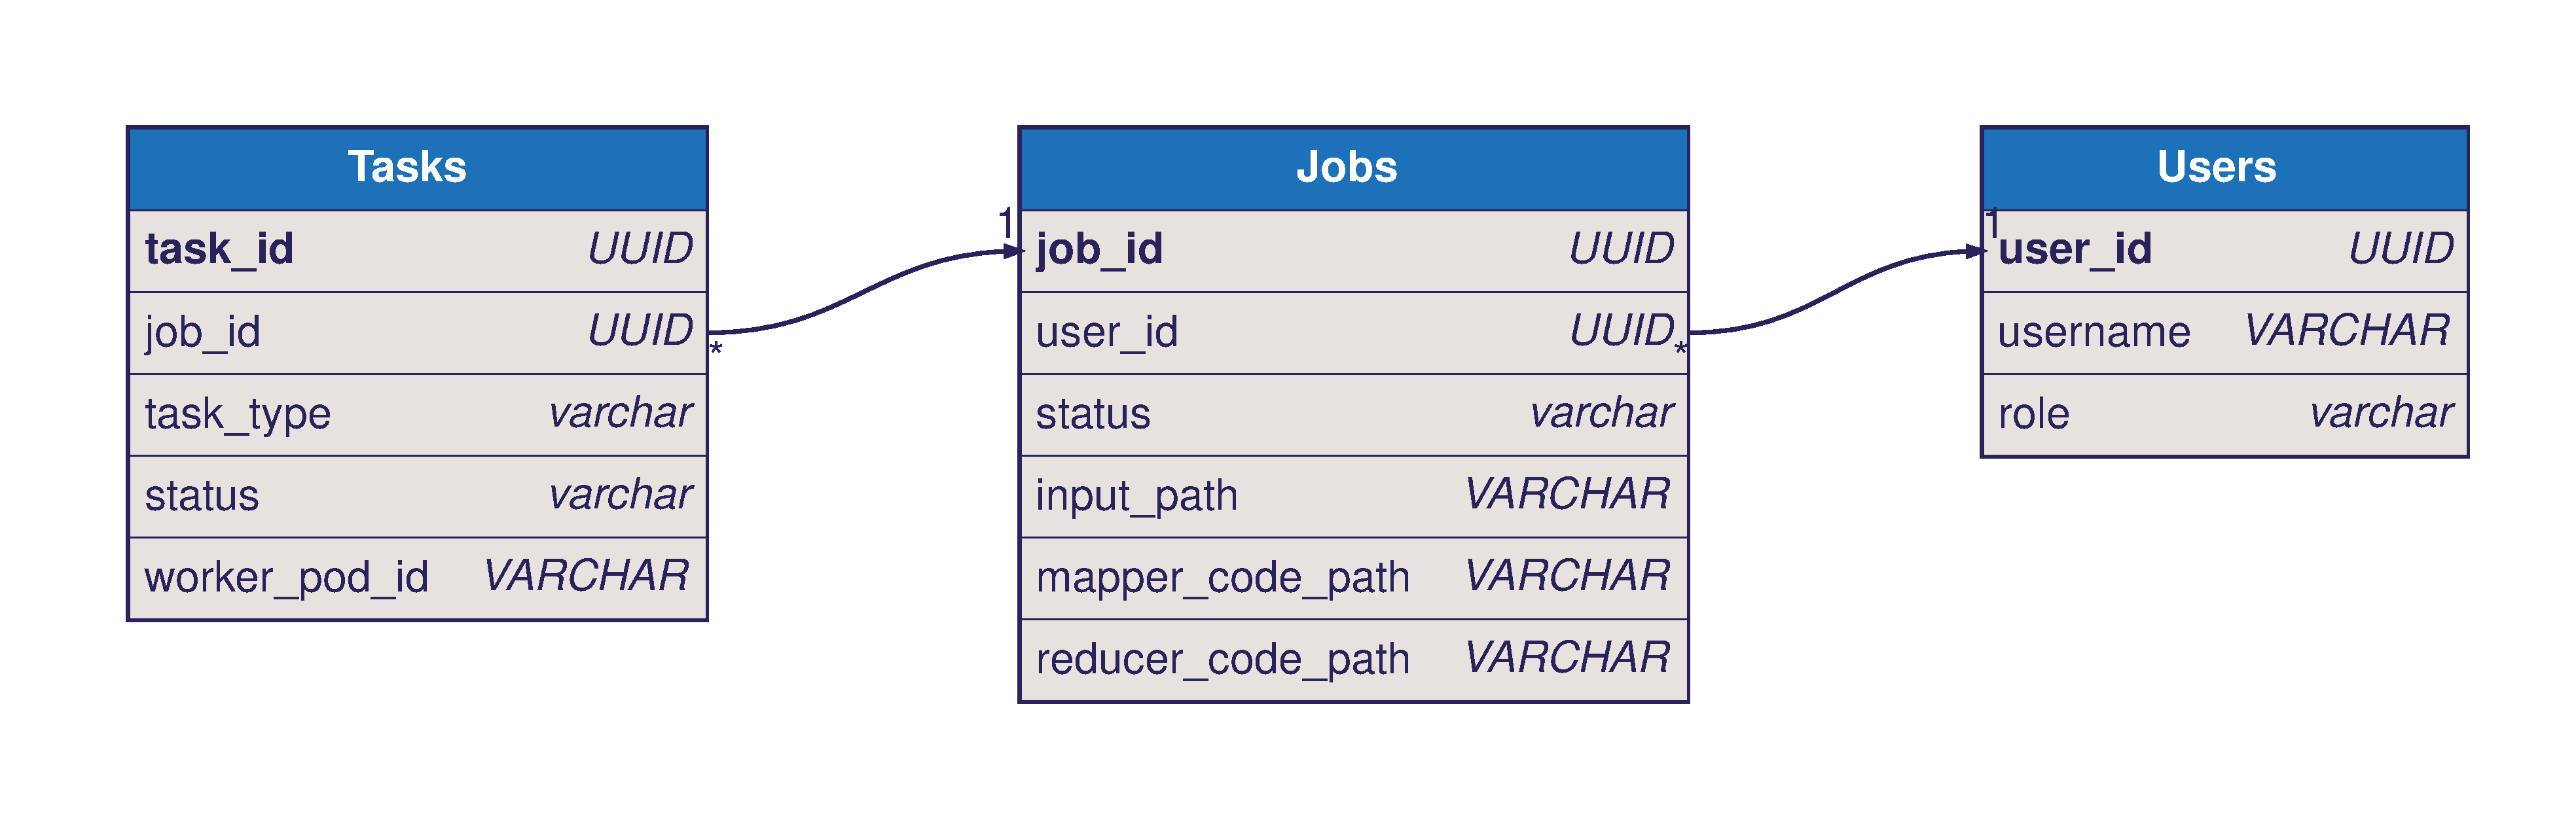
\includegraphics[width=0.7\textwidth]{diagrams/ER_Schema.pdf}
    \caption{Διάγραμμα Οντοτήτων-Συσχετίσεων (ER) της Βάσης Δεδομένων}
    \label{fig:er_schema}
\end{figure}

\vspace{0.5cm}

\begin{minipage}{\textwidth}
\noindent\textbf{Πίνακας: Users} \\
Αποθηκεύει τα στοιχεία των χρηστών του συστήματος και τους ρόλους τους.
\begin{center}
\renewcommand{\arraystretch}{1.2}
\begin{tabularx}{\textwidth}{|l|l|X|}
\hline
\rowcolor{LightBlue} % [ΠΡΟΣΘΗΚΗ] Χρωματιστή γραμμή κεφαλίδας πίνακα
\textbf{Πεδίο} & \textbf{Τύπος} & \textbf{Περιγραφή / Ιδιότητες} \\ \hline
\texttt{user\_id} & UUID & Primary Key \\ \hline
\texttt{username} & VARCHAR & Unique \\ \hline
\texttt{role} & ENUM & 'USER', 'ADMIN' \\ \hline
\end{tabularx}
\end{center}
\end{minipage}

\vspace{0.3cm}

\begin{minipage}{\textwidth}
\noindent\textbf{Πίνακας: Jobs} \\
Καταγράφει τα συνολικά Map-Reduce jobs που υποβάλλουν οι χρήστες.
\begin{center}
\renewcommand{\arraystretch}{1.2}
\begin{tabularx}{\textwidth}{|l|l|X|}
\hline
\rowcolor{LightBlue}
\textbf{Πεδίο} & \textbf{Τύπος} & \textbf{Περιγραφή / Ιδιότητες} \\ \hline
\texttt{job\_id} & UUID & Primary Key \\ \hline
\texttt{user\_id} & UUID & Foreign Key $\rightarrow$ Users \\ \hline
\texttt{status} & ENUM & 'PENDING', 'MAPPING', 'REDUCING', 'COMPLETED', 'FAILED' \\ \hline
\texttt{input\_path} & VARCHAR & Το URI του αρχείου δεδομένων στο MinIO \\ \hline
\texttt{mapper\_code} & VARCHAR & Το URI του αρχείου κώδικα (Python) στο MinIO \\ \hline
\texttt{reducer\_code} & VARCHAR & Το URI του αρχείου κώδικα (Python) στο MinIO \\ \hline
\end{tabularx}
\end{center}
\end{minipage}

\vspace{0.3cm}

\begin{minipage}{\textwidth}
\noindent\textbf{Πίνακας: Tasks} \\
Αναπαριστά τα επιμέρους κομμάτια (Map ή Reduce) ενός Job τα οποία ανατίθενται στους Workers.
\begin{center}
\renewcommand{\arraystretch}{1.2}
\begin{tabularx}{\textwidth}{|l|l|X|}
\hline
\rowcolor{LightBlue}
\textbf{Πεδίο} & \textbf{Τύπος} & \textbf{Περιγραφή / Ιδιότητες} \\ \hline
\texttt{task\_id} & UUID & Primary Key \\ \hline
\texttt{job\_id} & UUID & Foreign Key $\rightarrow$ Jobs \\ \hline
\texttt{task\_type} & ENUM & 'MAP', 'REDUCE' \\ \hline
\texttt{status} & ENUM & 'PENDING', 'RUNNING', 'COMPLETED', 'FAILED' \\ \hline
\texttt{worker\_pod} & VARCHAR & Το hostname του Kubernetes Pod που εκτελεί το task \\ \hline
\end{tabularx}
\end{center}
\end{minipage}

\end{document}